\documentclass{beamer}
\usetheme{Madrid}

\usepackage[utf8]{inputenc}
%\usepackage{beamerthemeshadow}
%\usepackage{stmaryrd} % Needed for \bigsqcap
%\usepackage{algorithm}
%\usepackage{algpseudocode}

%\definecolor{UBCblue}{rgb}{0.04706, 0.13725, 0.26667} % UBC Blue (primary)
\definecolor{Green}{rgb}{0.506, 0.727, 0.396} % UBC Blue (primary)

\usecolortheme[named=Green]{structure}


\newcommand\owlIndent{\hspace{4mm}}
\newcommand\setspacing{\hspace{2pt}}

\renewcommand{\arraystretch}{1.2} % Vertical spacing of rows in table


\begin{document}
\title{SubClass,Equivalence \& Existential Restrict.}  
\author{Henriette Harmse}
\date{}

\frame{\titlepage}
%\AtBeginSection[]
%{
%  \begin{frame}<beamer>
%    \frametitle{Outline}
%    \tableofcontents[]
%  \end{frame}
%}


\frame{\frametitle{Building Blocks of DLs and OWL}	
	\begin{table} 
		\begin{center} 
			\begin{small}
				\begin{tabular}{|p{1.75cm}|p{1.75cm}|p{1.75cm}|p{5cm}|} 
					\hline					
					\textbf{OWL}&\textbf{DL}&\textbf{Semantics}&\textbf{Example}\\
					\hline	
					instance or individual & instance or individual & A member of a set.	& A person called \texttt{Mary} or a dog called \texttt{Fido}.	\\
					\hline
					class & concept & A set of individuals.	& The \texttt{Person} class (concept) consisting of persons or the \texttt{Dog} class (concept) consisting of dogs. 	\\
					\hline
					object property & role & A set of pairs of individuals. & The \texttt{owns} object property (role) can link a pet and its owner: \texttt{Mary owns Fido} (in DL $owns(Mary, Fido)$).\\
					\hline
					data property & concrete role & A set of pairs where each pair consists of an individual linked to a data value. & The data property (concrete role) \texttt{hasAge} can link a number representing an age to an individual: \texttt{hasAge(Mary, 10) (in DL $hasAge(Mary, 10)$)} \\
					\hline  				  
				\end{tabular}
			\end{small}
		\end{center}
	\end{table}
}


\frame{\frametitle{The semantics of \texttt{SubClassOf}}
	\begin{block}{Syntax}
		\begin{table} 
			\begin{center} 
				\begin{small}
					\begin{tabular}{|c|c|c|} 
						\hline					
						\textbf{OWL}&\textbf{DL}&\textbf{Semantics}\\
						\hline 
						\begin{minipage}{4cm}
							$\begin{aligned}
								&\texttt{Class: C}\\
								&\owlIndent\texttt{SubClassOf: D}\\
								&\texttt{Class: D}
							\end{aligned}$
						\end{minipage}				
						& 
						\begin{minipage}{2cm}
							$\begin{aligned}
								C \sqsubseteq D
							\end{aligned}$
						\end{minipage}
						&
						\begin{minipage}{4cm}
							%trim option's parameter order: left bottom right top
							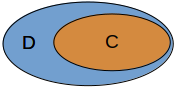
\includegraphics[trim = 0mm 0mm 0mm 0mm, clip, scale=0.4]{../../SubClassOf vs EquivalentTo/images/CsubClassOfD.png}
						\end{minipage}										
						\\
						\hline						 				  
					\end{tabular}
				\end{small}
			\end{center}
		\end{table}
	\end{block}
	\begin{block}{Semantics}
		The set $C$ is a subset of the set $D$. This means every individual of $C$ is necessarily an individual of $D$, but not every individual of $D$ is necessarily an individual of $C$.
	\end{block}
}


\frame{\frametitle{The semantics of \texttt{SubClassOf}}
	\begin{block}{Example}
		\begin{table} 
			\begin{center} 
				\begin{small}
					\begin{tabular}{|c|c|c|} 
						\hline					
						\textbf{OWL}&\textbf{DL}&\textbf{Semantics}\\
						\hline 
						\begin{minipage}{4cm}
							$\begin{aligned}
								&\texttt{Class: Dog}\\
								&\owlIndent\texttt{SubClassOf: Pet}\\
								&\texttt{Class: Pet}
							\end{aligned}$
						\end{minipage}				
						& 
						\begin{minipage}{2cm}
							$\begin{aligned}
								Dog \sqsubseteq Pet
							\end{aligned}$
						\end{minipage}
						&
						\begin{minipage}{4cm}
							%trim option's parameter order: left bottom right top
							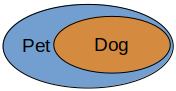
\includegraphics[trim = 0mm 0mm 0mm 0mm, clip, scale=0.4]{../../SubClassOf vs EquivalentTo/images/CsubClassOfDExample.png}
						\end{minipage}										
						\\
						\hline						 				  
					\end{tabular}
				\end{small}
			\end{center}
		\end{table}
	\end{block}
	\begin{block}{Guidance - When not to use}
		\begin{table} 
			\begin{center} 
				\begin{small}
					\begin{tabular}{|c|c|} 
						\hline					
						\textbf{When not use}&\textbf{Venn diagram}\\
						\hline 
						\begin{minipage}{6cm}
							When there is an individual of $C$ that is not an individual of $D$.
						\end{minipage}									
						& 
						\begin{minipage}{4cm}
							%trim option's parameter order: left bottom right top
							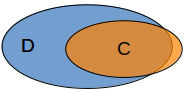
\includegraphics[trim = 0mm 1mm 0mm 1mm, clip, scale=0.4]{../../SubClassOf vs EquivalentTo/images/SubClassOfWhenNotToUse.png}
						\end{minipage}										
						\\
						\hline 
						\begin{minipage}{6cm}
							When every individual of $D$ is also an individual of $C$, then prefer using \texttt{EquivalentTo}.
						\end{minipage}									
						& 
						\begin{minipage}{4cm}
							%trim option's parameter order: left bottom right top
							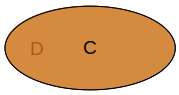
\includegraphics[trim = 0mm 1mm 0mm 1mm, clip, scale=0.4]{../../SubClassOf vs EquivalentTo/images/EquivalentTo.png}
						\end{minipage}										
						\\					
						\hline						 				  
					\end{tabular}
				\end{small}
			\end{center}
		\end{table}
	\end{block}
}

%\section{The semantics of \texttt{EquivalentTo}}
\frame{\frametitle{The semantics of \texttt{EquivalentTo}}
	\begin{block}{Syntax}
		\begin{table} 
			\begin{center} 
				\begin{small}
					\begin{tabular}{|c|c|c|} 
						\hline					
						\textbf{OWL}&\textbf{DL}&\textbf{Semantics}\\
						\hline 
						\begin{minipage}{5.25cm}
							$\begin{aligned}
								&\texttt{Class: C}\\
								&\owlIndent\texttt{EquivalentTo: D}\\
								&\texttt{Class: D}
							\end{aligned}$
							\smallskip\\
							\text{which can be seen as shorthand for:}
							\smallskip
							$\begin{aligned}
								&\texttt{Class: C}\\
								&\owlIndent\texttt{SubClassOf: D}\\
								&\texttt{Class: D} \\
								&\owlIndent\texttt{SubClassOf: C}\\
							\end{aligned}$					
						\end{minipage}				
						& 
						\begin{minipage}{2cm}
							$\begin{aligned}
								C \equiv D
							\end{aligned}$\\
							which can be seen as shorthand for
							\smallskip\\
							$\begin{aligned}
								C \sqsubseteq D \\
								D \sqsubseteq C
							\end{aligned}$					
						\end{minipage}
						&
						\begin{minipage}{2.75cm}
							%trim option's parameter order: left bottom right top
							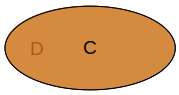
\includegraphics[trim = 0mm 0mm 0mm 0mm, clip, scale=0.4]{../../SubClassOf vs EquivalentTo/images/EquivalentTo.png}
						\end{minipage}										
						\\
						\hline						 				  
					\end{tabular}
				\end{small}
			\end{center}
		\end{table}
	\end{block}
	\begin{block}{Semantics}
		Every individual of $C$ is an individual of $D$, \textbf{and} every individual of $D$ is an individual of $C$.
	\end{block}
}




\frame{\frametitle{The semantics of \texttt{EquivalentTo}}
	\begin{block}{Example}
		\begin{table} 
			\begin{center} 
				\begin{small}
					\begin{tabular}{|c|c|c|} 
						\hline					
						\textbf{OWL}&\textbf{DL}&\textbf{Semantics}\\
						\hline 
						\begin{minipage}{4cm}
							$\begin{aligned}
								&\texttt{Class: Person}\\
								&\owlIndent\texttt{EquivalentTo: Human}\\
								&\texttt{Class: Human}
							\end{aligned}$
						\end{minipage}				
						& 
						\begin{minipage}{3cm}
							$\begin{aligned}
								Person \sqsubseteq Human
							\end{aligned}$
						\end{minipage}
						&
						\begin{minipage}{3cm}
							%trim option's parameter order: left bottom right top
							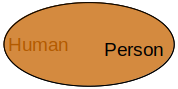
\includegraphics[trim = 0mm 0mm 0mm 0mm, clip, scale=0.4]{../../SubClassOf vs EquivalentTo/images/EquivalentToExample.png}
						\end{minipage}										
						\\
						\hline						 				  
					\end{tabular}
				\end{small}
			\end{center}
		\end{table}
	\end{block}
	\begin{block}{Guidance - When not to use}
		\begin{table} 
			\begin{center} 
				\begin{small}
					\begin{tabular}{|c|c|} 
						\hline					
						\textbf{When not to use}&\textbf{Venn diagram}\\
						\hline 
						\begin{minipage}{7.5cm}
							When there is an individual of $C$ that is not in $D$.
						\end{minipage}									
						& 
						\begin{minipage}{3cm}
							%trim option's parameter order: left bottom right top
							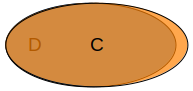
\includegraphics[trim = 0mm 0mm 0mm 0mm, clip, scale=0.4]{../../SubClassOf vs EquivalentTo/images/IndividualOfCnotInD.png}
						\end{minipage}										
						\\
						\hline 
						\begin{minipage}{7.5cm}
							When there is an individual of $D$ that is not in $C$.
						\end{minipage}									
						& 
						\begin{minipage}{3cm}
							%trim option's parameter order: left bottom right top
							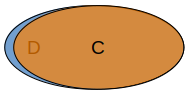
\includegraphics[trim = 0mm 1mm 0mm 1mm, clip, scale=0.4]{../../SubClassOf vs EquivalentTo/images/IndividualOfDnotInC.png}
						\end{minipage}										
						\\					
						\hline						 				  
					\end{tabular}
				\end{small}
			\end{center}
		\end{table}
	\end{block}
}

\frame{\frametitle{When to use \texttt{EquivalentTo} and \texttt{SubClassOf}}
	\begin{block}{\texttt{EquivalentTo}}
		\texttt{EquivalentTo} is used for definitions. That is when you want to state the necessary and sufficient conditions for a concept.
	\end{block}	
	\begin{block}{\texttt{SubClassOf}}
		\texttt{SubClassOf} is used when you want to define a hierarchy from the most general to the most specific. I.e., it is typically what you see in taxonomies
	\end{block}		
	
}

\frame{\frametitle{Qualified existential restrictions}
	\begin{block}{Syntax}
		\begin{table} 
			\begin{center} 
				\begin{small}
					\begin{tabular}{|c|c|c|} 
						\hline					
						\textbf{OWL}&\textbf{DL}\\
						\hline 
						\begin{minipage}{4cm}
							$\begin{aligned}
								&\texttt{ObjectProperty: r}\\
								&\texttt{Class: D}\\
								&\owlIndent\texttt{EquivalentTo:}\\
								&\owlIndent\owlIndent\texttt{r some C}\\
								&\texttt{Class: C}
							\end{aligned}$
						\end{minipage}				
						& 
						\begin{minipage}{1.5cm}
							$\begin{aligned}
								D \equiv \exists r.C
							\end{aligned}$
						\end{minipage}
						& 
						\begin{minipage}{4.5cm}
							%trim option's parameter order: left bottom right top
							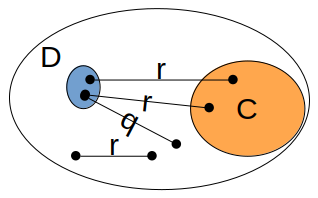
\includegraphics[trim = 0mm 1mm 0mm 1mm, clip, scale=0.4]{../../existential restrictions/images/QualifiedExistentialRestriction.png} 
						\end{minipage}															
						\\
						\hline						 				  
					\end{tabular}
				\end{small}
			\end{center}
		\end{table}
	\end{block}
	\begin{block}{Semantics}
		\begin{itemize}
			\item $(\exists r.C)^{\mathcal{I}} = \{x \in \triangle^{\mathcal{I}} | \text{there is an } y \in \triangle^{\mathcal{I}} \text{ such that } (x, y) \in r^{\mathcal{I}} \text{ and } y \in C^{\mathcal{I}}\}$
			\item \texttt{r some C} ($\exists r.C$) is the set of individuals such that for each individual $x$ there is at least 1 individual $y$ of type $C$ that is linked to $x$ via the object property (role) $r$.
		\end{itemize}
	\end{block}
}


\frame{\frametitle{Qualified existential restrictions}
	\begin{block}{Example using \texttt{EquivalentTo}}
		$\begin{aligned}
			&\texttt{ObjectProperty: owns}\\
			&\texttt{Class: PetOwner}\\
			&\owlIndent\texttt{EquivalentTo: owns some Pet}\\
			&\texttt{Class: Pet}
		\end{aligned}$
	\end{block}	
	\begin{block}{Example using \texttt{SubClassOf}}
		$\begin{aligned}
			&\texttt{ObjectProperty: owns}\\
			&\texttt{Class: DogOwner}\\
			&\owlIndent\texttt{SubClassOf: owns some Pet}\\
			&\texttt{Class: Pet}
		\end{aligned}$
	\end{block}		
	
}

\frame{\frametitle{Qualified existential restrictions}
	\begin{block}{Examples}
		Which of these individuals will be in \texttt{r some C} and therefore as well in \texttt{D}?\\
		\medskip
		\includegraphics[trim = 0mm 0mm 0mm 0mm, clip, scale=0.3]{../../existential restrictions/images/QualifiedRestrictionExamples.png}
	\end{block}	
	
	
	%trim option's parameter order: left bottom right top
	%	\includegraphics[trim = 63mm 0mm 0mm 20mm, clip, scale=1]{QualifiedRestrictionExamples.png} 
}


\frame{\frametitle{Qualified existential restrictions}
	\begin{block}{Examples}
		Which of these individuals will be in \texttt{r some C} and therefore as well in \texttt{D}?\\
		\medskip
		\includegraphics[trim = 0mm 0mm 0mm 0mm, clip, scale=0.3]{../../existential restrictions/images/QualifiedRestrictionExamples.png}
	\end{block}	
	
	\begin{block}{Answer}
		Individuals 2, 3, 5	
	\end{block}
}


\frame{\frametitle{Variations on existential restrictions}
	\begin{block}{Syntax}
		\begin{table} 
			\begin{center} 
				\begin{small}
					\begin{tabular}{|c|c|c|} 
						\hline					
						\textbf{Name}&\textbf{OWL}&\textbf{DL}\\
						\hline
						\begin{minipage}{1.5cm}
							Unqualified existential restrictions
						\end{minipage}
						& 
						\begin{minipage}{5cm}
							$\begin{aligned}
								&\texttt{ObjectProperty: owns}\\
								&\texttt{Class: Owner}\\
								&\owlIndent\texttt{EquivalentTo:} \\
								&\owlIndent\owlIndent\texttt{owns some owl:Thing}
							\end{aligned}$
						\end{minipage}	
						& 
						\begin{minipage}{4cm}
							$\begin{aligned}
								Owner \equiv \exists owns \top
							\end{aligned}$
							or\\
							$\begin{aligned}
								Owner \equiv \exists owns
							\end{aligned}$						
						\end{minipage}																		
						\\
						\hline	
						\begin{minipage}{1.5cm}
							Value restrictions
						\end{minipage}
						& 
						\begin{minipage}{5cm}
							$\begin{aligned}
								&\texttt{ObjectProperty: citizenOf}\\
								%&\owlIndent\owlIndent\texttt{citizenOf}\\
								&\texttt{Class: UKCitizen}\\
								&\owlIndent\texttt{EquivalentTo:} \\
								&\owlIndent\owlIndent\texttt{citizenOf hasValue UK} \\
								&\texttt{Individual: UK}
							\end{aligned}$
						\end{minipage}	
						& 
						\begin{minipage}{4cm}
							$\begin{aligned}
								UKCitizen &\equiv\\
								&\exists citizenOf.\{UK\}
							\end{aligned}$				
						\end{minipage}																		
						\\
						\hline	
						\begin{minipage}{1.5cm}
							Existential restriction on data property
						\end{minipage}
						& 
						\begin{minipage}{5cm}
							$\begin{aligned}
								&\texttt{DataProperty: name}\\
								%	&\owlIndent\owlIndent\texttt{name}\\
								&\texttt{Class: Person}\\
								&\owlIndent\texttt{SubClassOf:} \\
								&\owlIndent\owlIndent\texttt{name some xsd:string}
							\end{aligned}$
						\end{minipage}	
						& 
						\begin{minipage}{4cm}
							$\begin{aligned}
								Person &\sqsubseteq \\
								& \exists name.\texttt{xsd:string} 
							\end{aligned}$				
						\end{minipage}																		
						\\
						\hline															 				  
					\end{tabular}
				\end{small}
			\end{center}
		\end{table}
	\end{block}
}

\frame{\frametitle{Using existential restrictions with SubClassOf vs EquivalentTo}
	\begin{block}{A Person have 1 or more name}
	$\begin{aligned}
		&\texttt{DataProperty: name}\\
		%	&\owlIndent\owlIndent\texttt{name}\\
		&\texttt{Class: Person}\\
		&\owlIndent\texttt{SubClassOf:} \\
		&\owlIndent\owlIndent\texttt{name some xsd:string}
	\end{aligned}$\\
		\medskip
		Why did we use \texttt{SubClassOf} rather than \texttt{EquivalentTo}?\\
	\end{block}	
	
}

\frame{\frametitle{Using existential restrictions with SubClassOf vs EquivalentTo}
	\begin{block}{A Person have 1 or more name}
		$\begin{aligned}
		&\texttt{DataProperty: name}\\
		%	&\owlIndent\owlIndent\texttt{name}\\
		&\texttt{Class: Person}\\
		&\owlIndent\texttt{SubClassOf:} \\
		&\owlIndent\owlIndent\texttt{name some xsd:string}
		\end{aligned}$\\
		\medskip		
		Why did we use \texttt{SubClassOf} rather than \texttt{EquivalentTo}?\\
		\medskip
		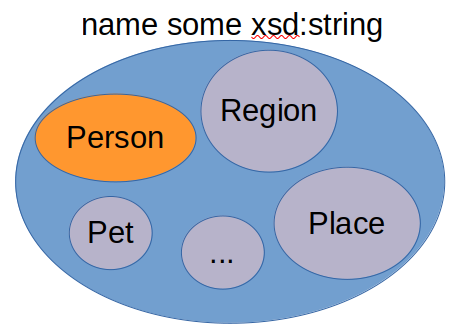
\includegraphics[trim = 0mm 0mm 0mm 0mm, clip, scale=0.3]{../../existential restrictions/images/ExistentialRestrictionsWithSubclassVSEquivalentTo.png}
	\end{block}	
}


\frame{\frametitle{Using existential restrictions with SubClassOf vs EquivalentTo}
	\begin{block}{A DogOwner is a Person that owns a Dog}
		$\begin{aligned}
			&\texttt{ObjectProperty: owns}\\
			&\texttt{Class: Dog}\\
			&\texttt{Class: Person}\\
			&\texttt{Class: DogOwner}\\
			&\owlIndent\texttt{EquivalentTo:} \\
			&\owlIndent\owlIndent\texttt{Person and owns some Dog} 
		\end{aligned}$
	\end{block}	
}



\end{document}
